% \documentclass[oneside]{report}
\documentclass[oneside,final,14pt,a4paper]{extreport}
% \documentclass[journal,onecolumn,a4paper,12pt]{IEEEtran}
\usepackage[T2A]{fontenc}


\usepackage{vmargin}
\setpapersize{A4}
\setmarginsrb{2.5cm}{2cm}{2cm}{2cm}{0pt}{10mm}{0pt}{13mm}
\usepackage{setspace}
\sloppy
\setstretch{1.5}
\usepackage{indentfirst}
\parindent=1.25cm

%%%%% ADDED TO SUPPORT TT BOLD FACES %%%%
\DeclareFontShape{OT1}{cmtt}{bx}{n}{<5><6><7><8><9><10><10.95><12><14.4><17.28><20.74><24.88>cmttb10}{}
\renewcommand{\ttdefault}{pcr}
%%%%% END %%%%%%%%%%%%%%%%%%%%%%%%%%%%%%% 
\usepackage{atbegshi,picture}
\AtBeginShipout{\AtBeginShipoutUpperLeft{%
  \put(\dimexpr\paperwidth-1cm\relax,-1.5cm){\makebox[0pt][r]{
\includegraphics[width=3cm]{figs/inno}}}%
}}


\usepackage[english]{babel}
\usepackage[backend=biber,style=ieee,autocite=inline]{biblatex}
\bibliography{ref.bib}
\DefineBibliographyStrings{english}{%
  bibliography = {References},}
\usepackage{blindtext}
\usepackage{pdfpages}
\newenvironment{bottompar}{\par\vspace*{\fill}}{\clearpage}
\usepackage{amsmath,amsfonts}

\usepackage{amsthm}
\newtheorem{theorem}{Theorem}
\newtheorem{corollary}{Corollary}
\newtheorem{lemma}{Lemma}
\newtheorem{proposition}{Proposition}
\theoremstyle{definition}
\newtheorem{definition}{Definition}
\theoremstyle{remark}
\newtheorem*{remark}{Remark}
\theoremstyle{remark}
\newtheorem*{example}{Example}



\usepackage{float}
\usepackage{graphicx}
\graphicspath{{figs/}} %path to images
\usepackage{array}
\usepackage{multirow,array}
\usepackage{caption}
\usepackage{subcaption}
\usepackage{hyperref}
\usepackage{paralist}
\usepackage{listings}
\usepackage{zed-csp}
\usepackage{fancyhdr}
\usepackage{csquotes}
\usepackage{color}

\usepackage{upgreek} 
\usepackage{bm}
\usepackage{hyperref}
\usepackage{setspace}
\usepackage{booktabs}
\usepackage{multirow}
\usepackage{longtable}
\usepackage[font=singlespacing, labelfont=bf]{caption}
\counterwithout{table}{chapter}
\renewcommand{\thetable}{\Roman{table}}
%Hints
\newcommand\pic[1]{(Fig. \ref{#1})} %Ref on figure
\newcommand\tab[1]{(Tab. \ref{#1})} %Ref on table


\usepackage{enumitem}
\newlist{inlinelist}{enumerate*}{1}
\setlist*[inlinelist,1]{%
  label=(\arabic*),
}




\pagestyle{fancyplain}

% remember section title
\renewcommand{\chaptermark}[1]%
	{\markboth{\chaptername~\thechapter~--~#1}{}}

% subsection number and title
\renewcommand{\sectionmark}[1]%
	{\markright{\thesection\ #1}}

\rhead[\fancyplain{}{\bf\leftmark}]%
      {\fancyplain{}{\bf\thepage}}
\lhead[\fancyplain{}{\bf\thepage}]%
      {\fancyplain{}{\bf\rightmark}}
\cfoot{} %bfseries


\newcommand{\dedication}[1]
   {\thispagestyle{empty}
     
   \begin{flushleft}\raggedleft #1\end{flushleft}
}

\begin{document}

% 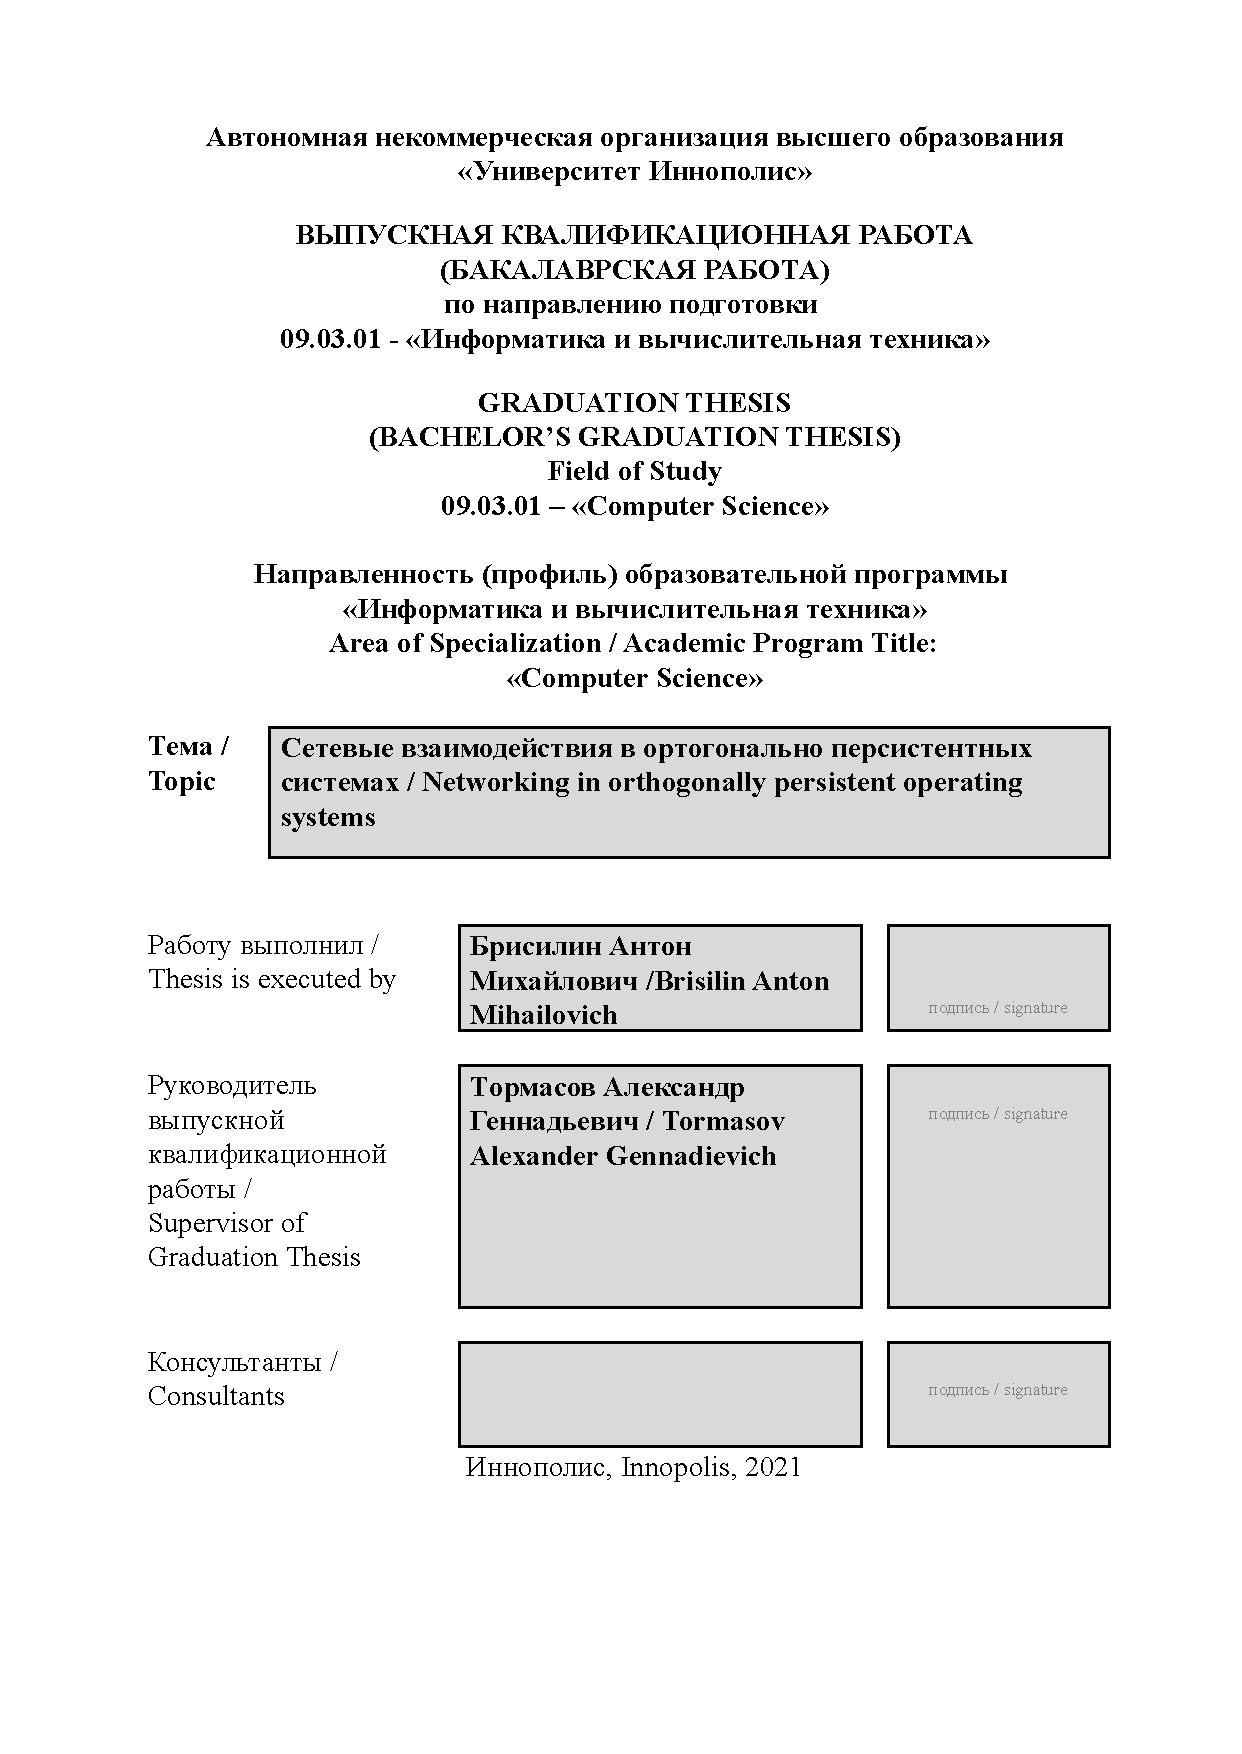
\includepdf[pages={-},offset=2.5cm -2cm]{title.pdf}
% \tableofcontents
% \listoftables
% \listoffigures


\newpage
% \begin{abstract}
abstract \ldots
\end{abstract}
% Depend on above part
% \setcounter{page}{6}
% \chapter{Introduction}
\label{chap:intro}
\chaptermark{Optional running chapter heading}
\section{Spacing \& Type}
\label{sec:section}

This is a section. This is a citation without brackets. and this is one with brackets \cite{A}. Multiple \cite{A,B,C} Here's a reference to a subsection: \ref{sec:subsection}. The body of the text and abstract must be double-spaced except for footnotes or long quotations. Fonts such as Times Roman, Bookman, New Century Schoolbook, Garamond, Palatine, and Courier are acceptable and commonly found on most computers. The same type must be used throughout the body of the text. The font size must be 10 point or larger and footnotes\footnote{This is a footnote.} must be two sizes smaller than the text\footnote{This is another footnote.} but no smaller than eight points. Chapter, section, or other headings should be of a consistent font and size throughout the ETD, as should labels for illustrations, charts, and figures.  

\subsection{Creating a Subsection}
\label{sec:subsection}

\subsubsection{Creating a Subsubsection}

\paragraph{This is a heading level below subsubsection}

And this is a quote: 
%
\begin{quote}
\blindtext
\end{quote}

\begin{figure}
\centering

\includegraphics[]{figs/inno.png}
\caption{One kernel at $x_s$ (\emph{dotted kernel}) or two kernels at
$x_i$ and $x_j$ (\textit{left and right}) lead to the same summed estimate
at $x_s$. This shows a figure consisting of different types of
lines. Elements of the figure described in the caption should be set in
italics, in parentheses, as shown in this sample caption.}
\label{fig:example}
\end{figure}

This is a table:
% currsize is not set in the long table environment, so we need to set it before we set it up.
\makeatletter
\let\@currsize\normalsize
\makeatother

% tabular environments are set to be single-spaced in the  thesis class,  but long tables do not use tabular
% to get around this, set the spacing to single spacing at the start of the long table environment, and set it back to double-spacing at the end of it

\begin{longtable}{cc}
\caption[This is the title I want to appear in the List of Tables]{This is a caption.} \label{tab:pfams} \\
\hline
A & B \\
\hline
\endfirsthead
\multicolumn{2}{@{}l}{\textbf{Table \thetable} \ldots continued} \\
\hline
A & B \\
\hline
\endhead
a1 & b1 \\
a2 & b2 \\
a3 & b3 \\
a4 & b4 \\
\hline
\end{longtable}


The package ``upgreek'' allows us to use non-italicized lower-case greek letters. See for yourself: $\upbeta$, $\bm\upbeta$, $\beta$, $\bm\beta$. Next is a numbered equation:
\begin{align}
\label{eq:name}
\|\bm{X}\|_{2,1}={\underbrace{\sum_{j=1}^nf_j(\bm{X})}_{\text{convex}}}=\sum_{j=1}^n\|\bm{X}_{.,j}\|_2
\end{align}
The reference to equation (\ref{eq:name}) is clickable. 
\section[Theorems, Corollaries, Lemmas, Proofs, Remarks, Definitions and Examples]{Theorems, Corollaries, Lemmas, Proofs, Remarks, Definitions,and Examples}

\begin{theorem}
\label{thm:onlytheorem}
\blindtext
\end{theorem}

\begin{proof}
I'm a (very short) proof.
\end{proof}

\begin{lemma}
I'm a lemma.
\end{lemma}

\begin{corollary}
I include a reference to Thm. \ref{thm:onlytheorem}.
\end{corollary}

\begin{proposition}
I'm a proposition.
\end{proposition}

\begin{remark}
I'm a remark. 
\end{remark}

\begin{definition}
I'm a definition. I'm a definition. I'm a definition. I'm a definition. I'm a definition. I'm a definition. I'm a definition. I'm a definition. I'm a definition. I'm a definition. I'm a definition. 
\end{definition}

\begin{example}
I'm an example.
\end{example}


\section[Optional table of contents heading]{Section with\\ linebreaks in\\the
name}


\Blindtext[2]





\chapter{Literature Review}
\label{chap:lr}
\chaptermark{Second Chapter Heading}

This chapter begins with an overview of the concept of persistence in general
and orthogonal persistence in particular in Section \ref{sec:lr:persistence}.
The Section \ref{sec:lr:networking} describes what special networking needs
do persistent systems have and then presents an overview of the TCP protocol,
which will be useful in next chapters. The last section of this chapter
briefly describes Phantom OS, Genode OS framework and the current state of
porting the former to the latter.

\section{Persistence}
\label{sec:lr:persistence}
\subsection{Persistence definitions}

The concept of \textit{data persistence} was informally introduced in Section
\ref{sec:intro-bg}. The formal definition of this concept is presented below.
\begin{definition}
The lifetime of a data is a time extent over which it can be used. This
lifetime is commonly called \textit{persistence} \cite{atkinson1983ps}. 
\end{definition}

Atkinson \textit{et al.} \cite{atkinson1995orthogonally,atkinson1983ps} give a
classification of application data by their persistence. This classification is
presented in Table \ref{tab:data_lifetimes}. As it was said earlier, the
support of levels 1-4 is usually provided by an operating system and a
programming language. This is due to the fact that these data are stored at the
main memory or lower memory levels. On the other hand, to have data with
persistence of levels 5-7, applications designers should rely on some external
component, such as database or file system. 

\begin{longtable}{cl}
\caption[Classification of data based on their lifetime]{Classification of data
based on their lifetime} 
\label{tab:data_lifetimes} \\
\hline
1. & Intermediate results in expression evaluation \\
2. & Local variables inside functions and code blocks \\
3. & Global variables and heap items \\
4. & Data that exists throughout a whole execution of a program \\
5. & Data that lasts for several executions of program \\
6. & Data that lasts for as long as a program is being used \\
7. & Data that outlives a program \\
\hline
\end{longtable}

\subsection{Orthogonal persistence}
\label{sec:LR:orth-persistence}

As was stated in section \ref{sec:intro-bg} using inherent programming
languages mechanisms and external mechanisms to access data interchangeably is
a burden for programmers. Presence of different data formats in each of these
storages makes this burden even heavier. As mentioned earlier, in response to
this problem, \cite{atkinson1995orthogonally} proposes to use persistent
support systems, which act as a mediator between supervised applications and
a transient environment. Atkinson \textit{et al.} also summarize design
requirements for such systems, which they call \textit{Principles of Orthogonal
Persistence}. The authors define the following requirements for an orthogonally
persistent support system: 

\begin{enumerate}
    \item The Principle of Persistence Independence. 
    
    Whether a program manipulates data that outlive it or not, the ways to use
    these data should be the same. There should be no significant difference in
    program syntax in either case.

    \item The Principle of Data Type Orthogonality. 
    
    Any part of data should be allowed to have any level of persistence, 
    irrespective of their type. There should be no special cases where objects
    of some type can not be persistent or transient.
    
    \item  The Principle of Persistence Identification. 
    
    The choice of how to identify which objects are persistent and how to
    provide persistence to them is not related to the universe of discourse of
    the system. The mechanism for identifying persistent objects should not also
    be related to the type system.

\end{enumerate}

A system that treats data according to these three principles is said to be
\textit{orthogonally persistent}. Two popular approaches exist to build such a
system. The first one is to integrate interactions with databases or file
systems into existing programming languages. In this case a program syntax to
access data stored in the memory should look the same as access to data in a
database. But semantics behind this syntax can vary. This idea is quite similar
to the work of modern Object-Relational Mapping (ORM) libraries
\cite{аннин2018краткий,copeland2008essential}. However, this approach is not
really orthogonally persistent since most ORM libraries put certain limitations
to what can be saved to the database. It also is sometimes problematic because a
different meaning behind seemingly similar fragments of code confuses
programmers.

The second approach is to build so-called \textit{persistent worlds} 
\cite{atkinson1995orthogonally}. These worlds usually have the form of an
operating system or a virtual machine. Applications residing in persistent
worlds are usually written with managed code. From now on I will use the term
\textit{persistent applications} for resident applications of persistent
worlds.

The fact that persistent applications are generally written with managed code
enables a system to automatically manage states of the applications so that they
have a consistent behavior across restarts. The examples of such systems are
KeyKOS \cite{bomberger1992keykos}, Grasshopper OS \cite{dearle1994grasshopper},
and Phantom OS. 

Creation of persistent support systems that work with nonvolatile memory (NVM)
as a main memory is an emerging research direction in the field of persistent
support systems. This approach seems to be more convenient for implementation
of orthogonally persistent systems, but it still has unsolved problems. The two
examples of such problems are the problem of dealing with changed states of
peripheral devices after restarts \cite{berthou2018peripheral}, and logical
problems with code execution \cite{ransford2014nonvolatile}. That is why the
creation of such systems is not a trivial question. 

\section{Networking in persistent systems}
\label{sec:lr:networking}

The nature of persistent applications implies that their execution can be
interrupted and then resumed after some time, when a host machine reboots. This
creates a challenge when an application is designed to communicate with remote
peers with a stateful network protocol. The challenge is to synchronize
states of the communicating peers: while a local system is offline a remote peer
can change a state of the connection indefinitely. Moreover, some persistent
support systems, like Phantom OS, use snapshotting to create an illusion of
uninterrupted execution. In case of such systems, the challenge is even more
problematic, because a persistent peer can "forget" that it had sent or received
some data. This happens if a record about data transfer was not embedded in a
snapshot, for example due to an unexpected power loss.

\subsection{Transmission control protocol}

The most popular transport layer protocol -- TCP -- is designed to provide a 
reliable packet delivery service. The reliability is achieved with periodic
retransmissions and acknowledgements. TCP packets are called segments. Each TCP
segment is equipped with two numbers - SEQ and ACK. SEQ, or \textit{sequence
number} is a number of payload bytes sent by the sender of the segment before
the current one. ACK, or \textit{acknowledgement number} stands for number of
payload bytes the sender received. To enhance the security and error tolerance
of the protocol initial SEQs are chosen randomly at the connection
establishment time. To enable error-detection TCP segments carry checksum that
comprises contents of the segment and so-called pseudo IP header
\cite{tcp_ip_illustrated_vol2}. The checksum can be updated incrementally,
without recomputing it for a whole packet \cite{rfc1624}.

When a host receives a TCP segment, the host's TCP checks the segment's SEQ
number. If SEQ is equal to $N$ and the last previously acknowledged byte had
number $N-1$ the segment is accepted and payload passed to the user of the TCP.
After the payload is queued to be delivered to the user, the receiving TCP
sends an acknowledgement segment with ACK equal to $N$.

TCP is a connection-oriented protocol. Before any data transmission happens,
communicating peers need to establish connection to negotiate transmissions
parameters. These parameters include exchange of initial SEQs. The connections
are established with a three-way handshake, that is, exchanging of three
segments - two from client to server, and one in the opposite direction.

TCP uses retransmissions and acknowledgements as follows. When a remote peer
does not acknowledge a packet TCP prescribes to retransmit it. The maximum
number of retransmissions is not stated in the original TCP specification
\cite{john1981transmission}.  However, the specification received updates
later, which prescribe to retransmit packets with exponentially increasing
delay \cite{rfc6298} until the timeout of at least 100 seconds \cite{rfc1122}.
This means that some TCP implementations will close a connection if their
peer appears to be down for more than 100 seconds.

The closing of connection when a host is temporarily offline is a good example
of a problem with traditional stateful protocols. The example highlights that
persistent support systems should restore the state of network connections in
the restoration phase when the execution was interrupted by a power loss.
Several approaches were proposed to hide closing of connections from user
applications.  The first approach, proposed by Ekwall, Urb{\'a}n and Schiper
\cite{ekwall2002robust}, is to create a session layer protocol that will behave
similar to the original TCP specification with respect to timeouts. That is,
the protocol will retransmit packets infinitely reopening underlying TCP
connections as they get closed.

The second approach was proposed by Zhang and Dao \cite{zhang1995persistent}.
This article, as well as the previous one, proposes to use a session-layer
protocol to create an abstraction of persistent connections, i.e. connections
that outlive execution of a one peer. The authors propose to use a centralized
notification service to transfer control messages. When this service detects
that a process goes down the service notifies all peers communicating with the
process. These processes switch their ends of connection to passive mode. In
this mode blocking read operations are getting blocked, and writes are buffered.
When the down process resumes its execution it registers in the notification
service. The former peers of the process receive this notification and try to
establish a connection to the continuation of the process. However, this
approach can lead to loss of data that were in flight when a process comes down.

Creation of a session-layer protocol on top of TCP is not the only way to
implement persistent connections. Zandy \textit{et al.} in \cite{rocks_racks}
propose a mechanism that hides disappearance of a remote peer from applications
that use TCP. The mechanism named \textit{rock} employs heartbeat probes via a
separate UDP control socket to detect if a remote peer is gone. When a process
detects loss of connection with a remote peer the process repeatedly tries to
reconnect to its peer by the last known physical address. If loss of a peer was
caused by network error, this will eventually succeed. Otherwise, the
reconnection attempt will be timed out. However, the rocks mechanism provide
a large timeout and it can be changed in per-connection basis, unlike TCP. 

To avoid loss of in-flight data while a process restarts a rock keeps a buffer
sized as a sum of local host send buffer size and peer host receive buffer
size. The buffer is used in a similar way as the send buffer is used in TCP:
the packets in the buffer are used to perform retransmissions.

\section{Phantom OS and Genode OS framework}
\subsection{Phantom OS}

Phantom OS is a general-purpose operating system, developed in 2009-2011. The
operating system consists of a stateless kernel and virtual machine, which
executes userspace applications. Phantom OS applications are written in Phantom
programming language. The execution of managed code is persistent, which makes
Phantom OS a persistent support system. As was said earlier, persistence for the
managed code is achieved using snapshotting. Phantom is an experimental system,
in a sense that it is developed as a proof-of-concept and is not ready for
production use.

Phantom OS currently supports only i386 ISA and it has all drivers embedded 
inside a kernel. It is problematic, because to support wide range of hardware
OS needs drivers, which is often delivered by third-party developers. But in
case when drivers are embedded in kernel an error in driver can crash the whole
system. Implementation of drivers as parts of kernel also complicate
development and delivery of the drivers.

These are two reasons why it is desirable to replace Phantom kernel with a
microkernel. The port of Phantom OS to the Genode OS framework is being
developed right now. It is implemented as a Genode component running the PVM.
This means that network capabilities are provided by the Genode level of the
PoG port.  That is why I will concentrate my attention on development of a
network stack working in Genode.

\subsection{Genode OS framework} 
The Genode OS Framework \cite{genode_foundations} is a toolkit for creating 
operating systems. It provides a possibility to build a microkernel operating
system from set of existing components. Genode also provides an API to
integrate various microkernels into it.

For now the supported kernels include Linux kernel, nova microhypervisor and
several kernels from the L4 kernel family. Supported kernels from the last
family include L4ka::Pistachio, Fiasco.OC, formally verified seL4 microkernel,
and L4/Fiasco.  The framework also supports execution on bare hardware on ARM
and x86-64 ISA.

The Genode itself provides mechanisms for threading and synchronisation,
inter-process communication (IPC), virtual memory, pluggable device drivers,
sandboxing, and VFS. Processes in Genode are called \textit{components}. Genode
components usually belong to one of the five categories: device drivers,
resource multiplexers, protocol stacks, applications and runtime environments
\cite{genode_foundations}. Genode's VFS with possibility of adding custom
plugins to it. For instance, the ram-fs plugin can expose a part of process
memory as a file. This is particularly convenient when one uses libc that has
an API that is mostly file-oriented. TCP/IP stacks are also implemented as VFS
plugins that represent each socket as a set of files. VFS plugins are merely
shared libraries that are loaded by VFS at runtime. Genode applications are not
linked with VFS plugins.

Genode's IPC mostly consists of blocking remote procedure calls (RPC). To use
an RPC object provided by a server component, a client component should have a
\textit{capability} to call it. A capability is a special reference to an RPC
object which is backed by the kernel. Possession of capability is enough to use
an object that it references to. Capabilities are typed with the RPC interface
they provide. Genode components have capability quotas - maximum number of
capabilities they can own.

Genode TCP stacks use the Network interface card (Nic) RPC interface as an
input and output. That is, TCP stacks submit and receive packets via these
interfaces. The Nic interface is implemented by a regular userspace component
and therefore its implementation can be changed on a per-component basis.

Genode VFS plugins and Genode components in general are not persistent. TCP
stacks lose their state after a power loss. Therefore, I need to implement
saving and restoring of state of a TCP stack before it can be used by PVM.

% \chapter{Methodology}
\label{chap:met}


\ldots

Referencing other chapters \ref{chap:lr}, \ref{chap:met}, \ref{chap:impl}, \ref{chap:eval} and \ref{chap:conclusion}

\ldots
% \chapter{Implementation}
\label{chap:impl}


\ldots

% \chapter{Evaluation and Discussion}
\label{chap:eval}


\ldots

% \chapter{Conclusion}
\label{chap:conclusion}


\ldots



%% REFERENCES
% \printbibliography[heading=bibintoc,title={Bibliography cited}]
% \appendix
\chapter{Implementation}
This section contains source code fragments used in discussion of
implementation.  

\section{Example configuration for Genode component with networking
capabilities}
\label{appex:conf-sample}

\begin{lstlisting}
<start name="test" caps="100" priority="-1">
  <resource name="RAM" quantum="50M"/>
  <config>
    <vfs>
      <dir name="socket"> <ptcp dhcp="yes"/> </dir>
    </vfs>
    <libc socket="/socket"/>
  </config>
</start>
\end{lstlisting}

\end{document}